\chapter{Movement}\label{ch:movement}

\begin{wrapfigure}{R}{0.3\textwidth}
    \centering
    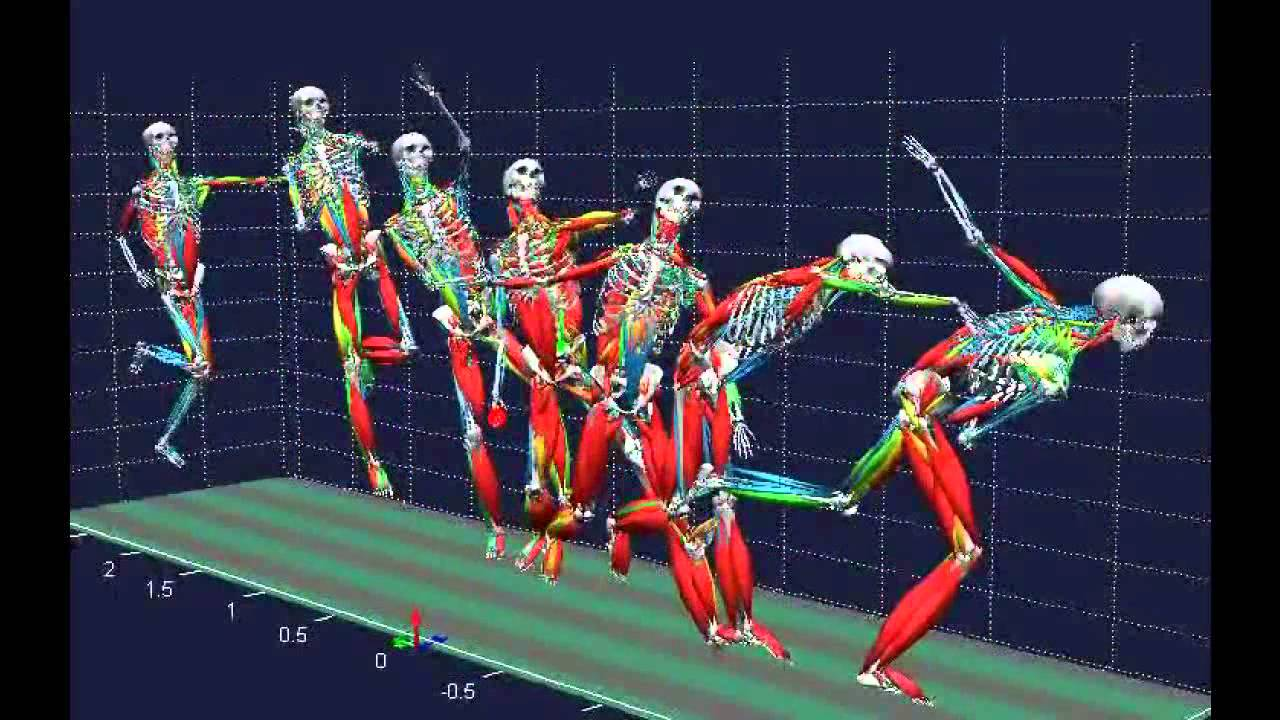
\includegraphics[width=0.25\textwidth]{images/movement}
\end{wrapfigure}

This chapter is based on the previous ones about anatomy/physics, and how these concepts give raise to higher concepts we encounter while practicing CI\@.
We will take a look at the fascinating science of movement, movement theory and a bit of biomechanics, and also deal with more abstract views on movement as maybe known from the dancing world.
For more experienced (improvisation) dancers, a lot of the things mentioned here might sound familiar, for the more inexperienced among us this can open a totally new perspective on movement.

\section{Movement Qualities}\label{sec:movement-qualities}

There are different imagined \textbf{dimensions} we can play with, to tap into different qualities on how to use our body, giving it a different flavor, allowing us to do different techniques, and by knowing the pros and cons of each quality, we can apply them in the right moment to elevate our technical skill and also keep things safe for ourselves and our partner.

\begin{itemize}
    \item [] \textbf{Muscle Tone} \\
    We can play a lot with tone, which is the amount of tension we create in our muscles that makes us either more relaxed or more stiff.
    In general, we prefer to maintain the least amount of effort, a minimum muscle tension; as little as possible, as much as necessary.
    By being more relaxed, we are more flexible, can adapt to an ever-changing situation, and also are more receptive via our tactile sense, being able to receive more information, to listen better.
    To have some images to play with, think of moving through air (well, you don't have to imagine that, as we constantly do that --duh).
    Instead, think of you being a cloud, floating through the sky (sure, that's better, we usually never do that one).
    Now increase tension by imagining moving through water, how it creates a small but continuous resistance, preventing you from sharp, edgy movements, from breaking a fluent pathway.
    The next increase in resistance could be achieved by imagining something like honey, sticky and slowing down your movements, having you to add more muscle effort.
    And as a final step, imagine being stuck in concrete, which maybe has not yet fully harden, still making you almost unmovable.

    \item [] \textbf{Speed} \\
    Moving on to the very obvious dimension of slowness and fastness.
    The slow can be extremely slow, to gain lots of information of internal sensations.
    The fast can be released in an explosive manner, like a shockwave through the whole body.
    Both, and everything in-between, can be alternated rapidly, to gain more control (of speed).

    \item [] \textbf{Kinesphere} \\
    The degree of extension of the limbs into the space --without stepping-- is called \gls{kinesphere} with which we can play with.
    We could segregate it into a small (body), medium (elbows, knees), large (wrists, ankles) and extra large (fingers, toes), and something more abstract going even beyond (projecting outwards), the universe.
    Each of them is creating a differently sized ball, or more like an egg shape, around us in which we are limited to move within and also want to stay in constant contact with.

    \item [] \textbf{Levels} \\
    Next to extension into space, we can, of course, take different levels in vertical space: Up (standing), middle (hinged, or on hands and knees being a ``little animal'') and floor work (lying on the ground).
    With the help of relaxation and tension, we can quickly change our position on the vertical axis and play with explosive dynamics.
    Also, mirroring your dance partner, staying at a different (not the same as with imitating) level then he, can be an challenging, fun, and engaging expierence to explore.

    \item [] \textbf{Isolation} \\
    The isolation of certain body parts can also be fun --and challenging at the same time-- to play with.
    The most simple one is to divide the body into upper and lower, left and right side, same side or cross side (homo- or contra-lateral, see the anatomy section for explanation of terminology), or move only in a certain plane.

    \item [] \textbf{Shapes} \\
    The forms we are drawing in air can be another dimension.
    Think of straight lines (edgy, staccato) versus roundness (flowy, fluid, air).
    People who have experience with the practice of 5 Rhythms might be familiar with those concepts and make use of them.
\end{itemize}

To bring those qualities to a next level, try to \textbf{combine} them in different ways.
Often slow, fluid and soft go together, but how about changing one of them to the other extreme?!
Or the legs are in the large kinesphere being soft and staccato, while the arms in the small kinesphere and hard and fluid.
Have a partner telling you what parts should be in which quality, to surprise yourself by finding combinations you would not have thought of alone.

\section{Partner Dance}\label{sec:partner-dance}

\textit{Disclaimer}: There is lots to tell about dancing with one (or more) partner(s), and this subsection will be far from mentioning all the most relevant there is, but ought to give just a quick glimpse of what might be encountered at the beginning of your CI journey.

Humans are \textbf{social animals}, and as such we have countless neuronal networks dedicated to processing social information, hardwired bonding tendencies leading to the ability to read each other, get in-tuned with each other, ultimately leading to harmony in groups.
Think of basic empathy, which is associated to mirror neurons in our brain, which for example leads us to yawn once we see someone else yawning, or feel the pain we observe in that funny (?) video clip where someone falls from a skateboard.
If we want to feel how someone else is feeling, we might simply want to put our full presence with that person (or even a group) and feel inside our bodies of what's happening; there is a high chance that what we experience is the other person's state of being.
Using a more ``flowery language'', we could say that this is the ability of ``\textit{feel the other person's energy}'' --whatever is supposed to be meant by (mis-)using the word ``energy'' here.

As human beings we also have the innate need to \textbf{be seen} by others; being ignored as one of the worst punishments we can experience, leading to feelings of isolation, exclusion and loneliness.
The biggest present therefore we can give each other is to \textbf{mirror} each other's movements; explicitly acknowledging the other person's existence, putting one's attention to that person, copying his movements, which is also called ``\textit{kinesthetic resonance}''.
Of course counter-mirroring has the same effect (you go down, I go up; you go left, I go right), as it still maintains a form of connection we can play with.

\section{Body Awareness}\label{sec:body-awareness}

Let's have a look of how we actually become aware of our bodies.
The biological and physiological base of how this fascinating organic machinery --roughly-- works.

\subsection{Vestibular System}\label{subsec:vestibular-system}

This is our sense of \textbf{balance} and spatial orientation for the purpose of movement coordination, and is all well known to us.
It consists of two components: The (three, as there are three dimensions) \textit{semicircular canals} for rotational movements, and the \textit{otoliths} for linear accelerations.
Signals from those are sent to the muscles to keep us upright and control posture, allowing us to maintain our desired position in space.
Together with our proprioception, we can understand our body's dynamics and kinematics in any given moment.

\subsection{Proprioception}\label{subsec:proprioception}

\Gls{proprioception} allows us --as a sort of 6th sense, the ``kinesthetic sense''-- to be consciously aware of movement, force and body \textbf{position}.
It tells us our body's position in the space, that is the relative positioning of neighboring body parts, and the strength of effort needed for movement.
Try for example to close your eyes and touch your nose; you will be able to do this without looking (in a mirror, or in complete darkness) because of little cells (little \textit{spindles} which are spring-like protein molecules which are stretched inside your muscles) in your body being aware of the \textbf{amount of stretch} they experience (joint position sense), which is then processed subconsciously by your brain giving raise to a bodily sensation.
Everyone is familiar with the knee-jerk reflex, where the patellar tendon is rapidly stretched to an extreme (usually with the help of a hammer), which leads to an immediate response (a reflex) to counteract that and protect the tissue from injury.

Related sensations are \textit{exteroception}, the perception of the outside world, and \textit{interoception}, the perception of internal sensations like pain and hunger.

\subsection{Kinesthesia}\label{subsec:kinesthesia}

\Gls{kinesthesia} is the awareness of position and \textbf{movement} of body parts using sensory organs (proprioceptors, mechanosensory neurons) in muscles, tendons and joints.
It's crucial in muscle memory and hand-eye coordination.
Sometimes it's confused with proprioception, but those two are different concepts.
If you have an inner ear infection for example, and the sense of balance is affected, this would degrade the proprioceptive, but not the kinesthetic sense.
Moreover, proprioception is more about joint position (more subconscious cognitive awareness of your body in space and balance) whereas kinesthesia is more about awareness of joint movement (more conscious body's motion, behavioral).

\subsection{Neuronal Processing}\label{subsec:neuronal-processing}

\textbf{Neuromuscular control} is the efferent (signal from the central nervous system to the body) response to an afferent (sensory) input, which is the functional component to movement and athletic activities that is referred to as dynamic stability.
Sensory input comes as (different types of\footnote{The four mechanoreceptors are: Meissner corpuscle for heavy pressure, Pacinian corpuscle for vibraiton, Merkel disks for light touch and Ruffini endings for skin stretch}) \textbf{mechanoreceptors} located in muscles, capsules and ligaments, allowing us awareness of joint position, movement, and acceleration.

All that information (vestibular, proprioceptive, kinesthetic) including the visual input is sent to the brain, where it is processed and integrated to allow us to create an overall representation of body position, movement and acceleration.

\section{Space Harmony}\label{sec:space-harmony}

This movement theory --and practice, also called \textit{Choreutics}-- was developed by the Austrian-Hungarian dancer and choreographer Rudolf Laban, to study the natural sequences of movements we follow in daily life; studying ``the art of movement'' to recognize spatial patterns.

When dancing, the term \textbf{\gls{kinesphere}} is used to refer to the space immediately reachable by your limbs without changing your place on the ground.
We can use up a lot of that space within this sphere (\textit{Far Reach Kinesphere}), just a bit (\textit{Near Reach Kinesphere}) or something in-between (\textit{Mid Reach Kinesphere}).

\begin{wrapfigure}{R}{0.3\textwidth}
    \centering
    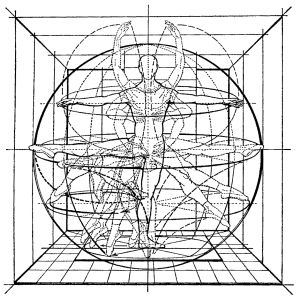
\includegraphics[width=0.25\textwidth]{images/kinsphere}
    \caption{The \textbf{kinesphere} around the body reachable by extended limbs.}
\end{wrapfigure}

Furthermore, Mister Laban believed that there are three types of movers which prefer different \textbf{levels}: Those who enjoy leaping and springing off the ground move in \textit{High Level}, those with more sensuous movement enjoying the \textit{Central (Middle) Level}, and those who prefer more earth-bound movements who stayed in the \textit{Deep (Low) Level}.

Within the kinesphere we can move from one point to another through different approaches, so-called \textbf{pathways}: When movement is initiated from (or passes through) the body's center we take the \textit{Central Pathway}, along the outer limits of the kinesphere it takes a \textit{Peripheral Pathway}, and when the movement passes between center and periphery it takes a \textit{Transverse Pathway}.

There is of course much more to say about this, including the Laban Movement Analysis (LMA) which is a method and language for describing, visualizing, interpreting, and documenting movement, but this would go beyond the purpose of this book.
